%
% fig-zweipunkte.tex -- analytische Fortsetzung für zwei Punkte
%
% (c) 2026 Prof Dr Andreas Müller
%
\begin{figure}
\centering
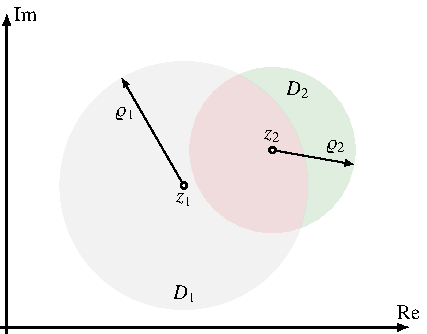
\includegraphics{chapters/040-analytisch/images/zweipunkte.pdf}
\caption{Die Potenzreihe einer auf dem Kreis um $z_1$ mit Radius
$\varrho_1$ definierte holomorphe Funktion $f_1(z)$ kann im Punkte
$z_2$ in eine neue Potenzreihe $f_2(z)$ mit Konvergenzradius
$\varrho_2$ entwickelt werden.
Im roten Teilgebiet stimmen die Funktionen überein.
Im grünen Teilgebiet ist die Funktion $f_2(z)$ die einzig mögliche
holomorphe Erweiterung der Funktion $f_1(z)$.
\label{buch:analytisch:fig:zweipunkte}}
\end{figure}

